\section{ODE Analysis}

The ODE system obtained by removing the spatial term in equation ~\ref{eq::nondimyM} can exhibit a variety of behaviours numerically (Fig. ~\ref{fig::odeanal}). 
\begin{figure}[h]
\centering
\captionsetup{width=\linewidth}
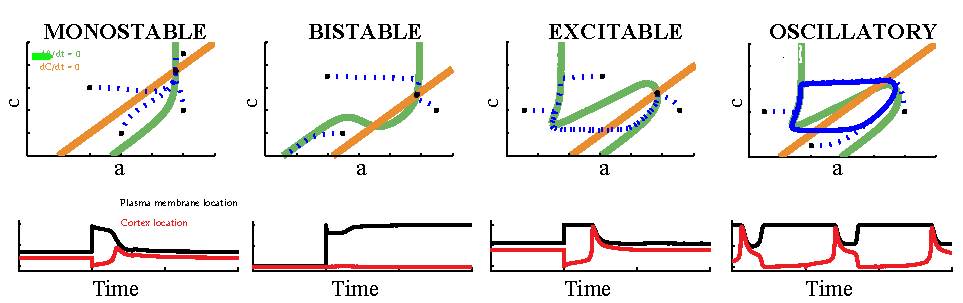
\includegraphics[width=4.5in]{Project2/figs/ODE_Analysis.pdf}
\caption{odes.}
\label{fig::odeanal}
\end{figure}

We swept through two parameters, $\epsilon$ and $\Omega$, in order to study the transitions between these behaviours, see Fig. ~\ref{fig::epsomega}. We note that the oscillatory behaviours of the ODE system is dependent on the fast-slow dynamics established by small values of $\epsilon$. The second transition into the oscillating regime, along decreasing values of $\Omega$,  occurs in conjuction with a canard explosion, as the system seem to jump from a single steady state solution to large amplitude oscillations with a small change in the parameter. This is a known feature exhibited by somefast-slow dynamical systems[REFERENCE].

\begin{figure}[h]
\centering
\captionsetup{width=\linewidth}
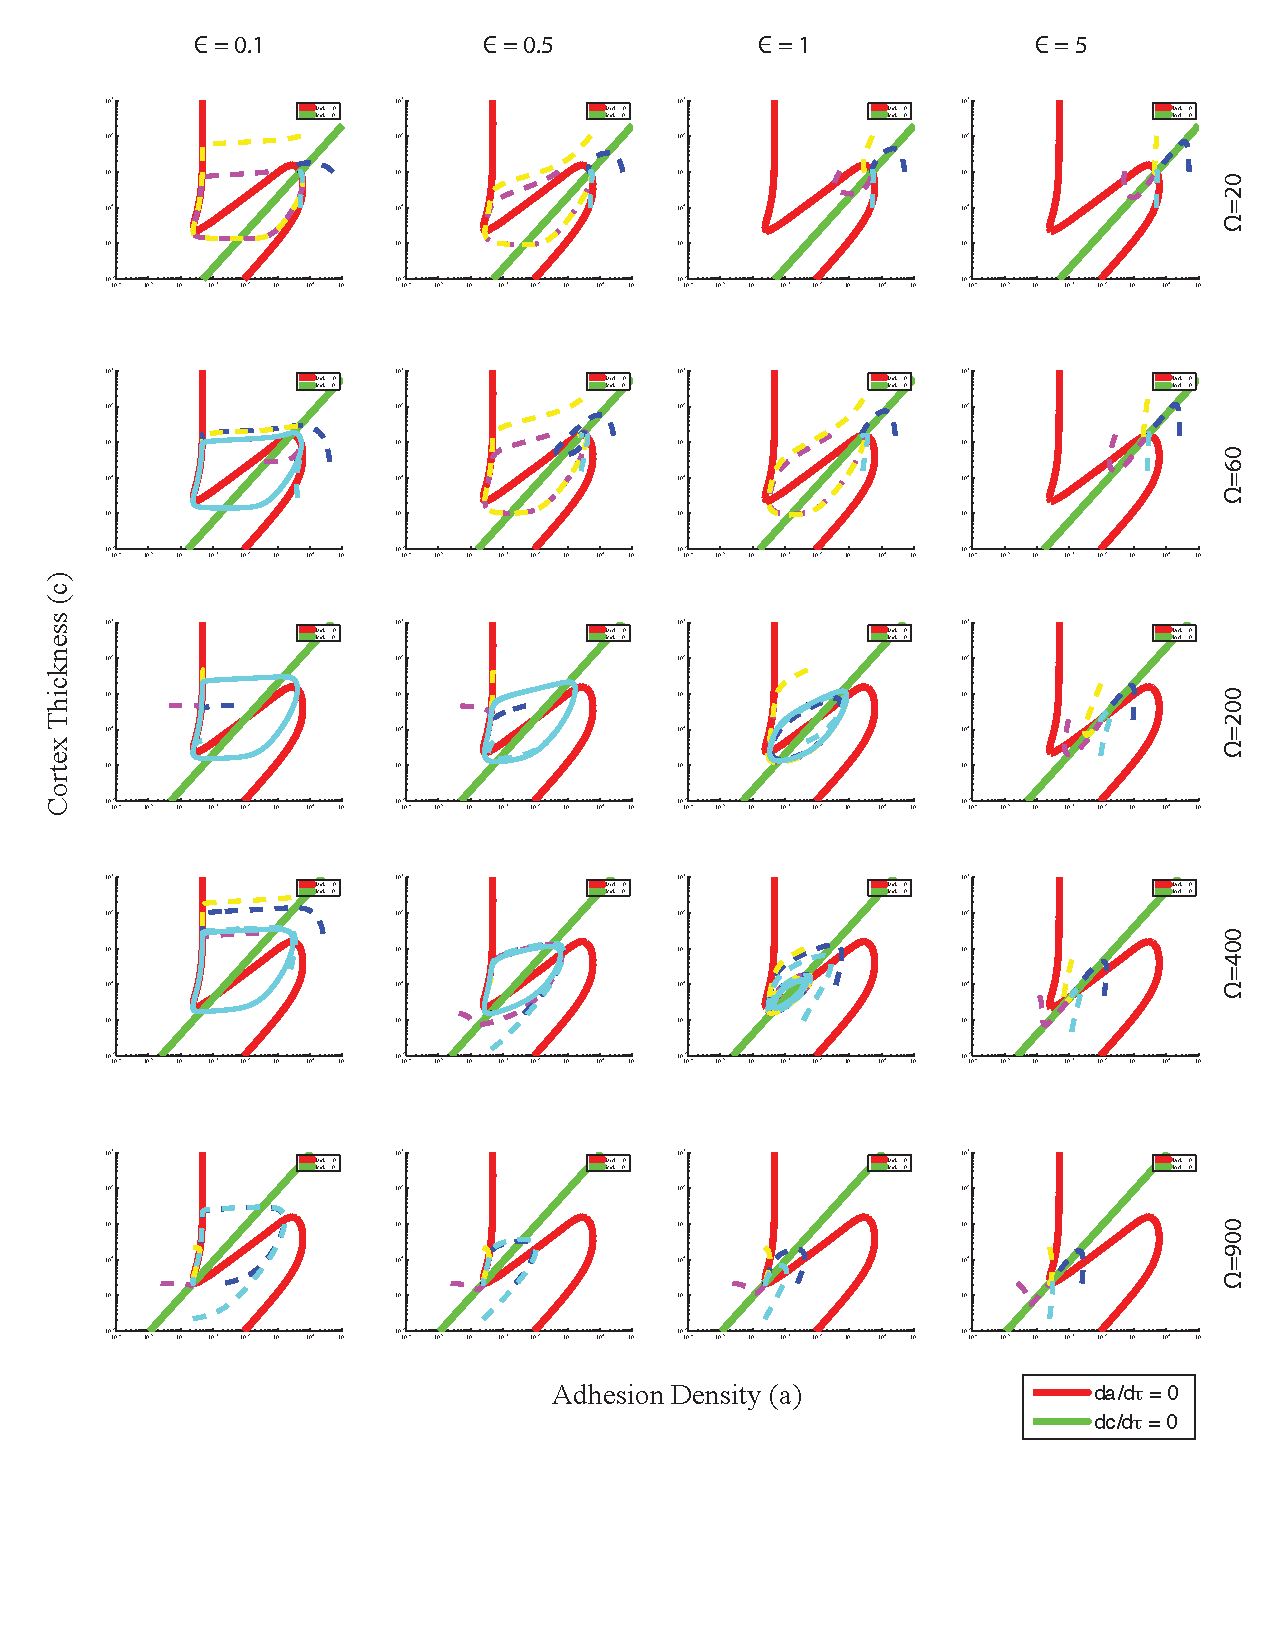
\includegraphics[width=4.5in]{Project2/figs/Epislon_omega.pdf}
\caption{two parameter bif.}
\label{fig::epsomega}
\end{figure}
 
 We plan to do a two parameter bifurcation analysis to characterize the bifurcation lines and further explore the so-called {\textit{canard}} point at which the oscillations appear to jump. The resulting bifurcation diagram might look something like Fig. ~\ref{fig::bifplot}. 

\begin{figure}[h]
\centering
\captionsetup{width=\linewidth}
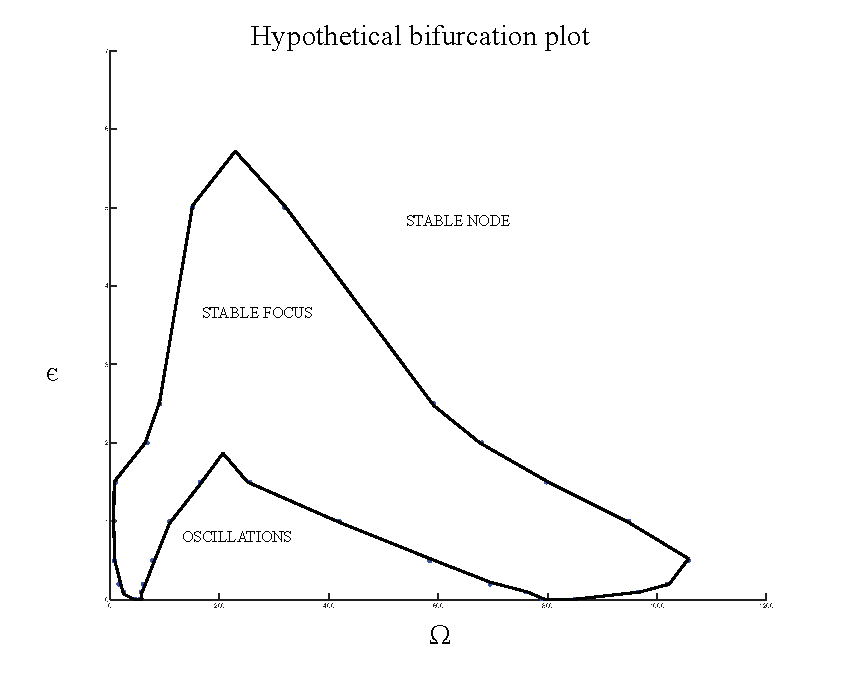
\includegraphics[width=4.5in]{Project2/figs/Hypothetical_bifurcation_plot.pdf}
\caption{two parameter bif.}
\label{fig::bifplot}
\end{figure}

